We evaluate our intersection of unions method on three examples, i.e.,
1) The illustrative Example~\ref{eg:ill} 2) A seven dimensional model
of autonomous car with one input proposed in~ 3) A twelve dimensional
model of quadrotor from ARCH workshop~.  For the illustrative example,
we compare the flowpipe accuracy of our method with that of only
\emph{union of zonotopes} based on the performance index in
Equation~\ref{eqn:pi} proposed by Althoff
et.al.~\cite{althoff2008reachability} .  On the other two real world
examples, besides the performance index~(\ref{eqn:pi}), we compare our
method with state-of-the-art methods, i.e., polynomial
zonotopes in CORA and Taylor models in Flowstar.  We obtained a high
increase in flowpipe accurary compared to other methods.

For computation of symbolic derivatives, we use Sympy Python software and for
interval arithmetic, we use Boost C++ library.  Main parts of
our algorithm are parallelizable, so we gain significant speed by
running on mulicore machines.

\subsection{Illustrative example}
We consider the 3-dimensional nonlinear system in Example~\ref{eg:ill}
to illustrate the difference in accuracy between our IoU flowpipe and
the union flowpipe based on the performance index
in~\cite{althoff2008reachability}(~\ref{eqn:pi}).  The initial set has
to be large enough to demonstrate the effect of linearization error.  We
take this as $X_0 = [-1,1]^3$.
\paragraph{Settings:}  We tested this example on a 1.4 GHz
laptop with 4 GB ram, 1600 MHz DDR3 with 4 virtual cpu cores.  We ran
our intersection of unions flowpipe algorithm and the only union
flowpipe~\ref{eqn:pi} algorithm for 3 different number of divisions,
$2^\eta:\eta = 2, 3,4$, i.e., $4, 8$ and $16$ divisions. The order of
interval zonotope is $l = 200$ and the time step size is $\delta =
0.01\si{\second}$.  Furthermore, $\epsilon = 10^{-12}$ and $K = 20$.

\paragraph{Results:}  The upper and lower bounds on flowpipes at uniformly spaced time
points as well as the overall bounds on the $x$ and $y$ variables are
shown in Figure~\ref{fig:ill}.  The figure clearly demonstrate our IoU
method to be far more accurate than the union method on $x/y$
coordinates.  The bounds for $\theta$ are almost similar for both
methods and all types of divisions because of very less linearization
error $(\le 10^{-6})$.  The computation times for our IoU method are $6\si{\second}$, $12\si{\second}$ and $24\si{\second}$, respectively, for $4$, $8$ and $16$ divisions
per union.  The computation times will reduce significantly by using
more cpu cores, which would be useful for the higher dimensional
examples that we evaluate latter.
%
\begin{figure}
  \includegraphics[scale = 0.7]{illImages/Ub.png}
  %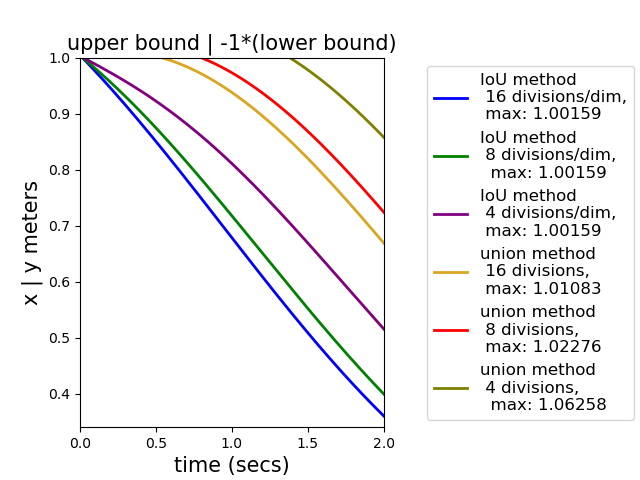
\includegraphics[scale=0.5]{illImages/ub.png}
  \caption{Flowpipe bounds at different time points for
    Example~\ref{eg:ill}}
  \label{fig:ill}
\end{figure}
%

